% TEX program = xelatex
% compile: xelatex -> biber/bibtex -> xelatex -> xelatex
\documentclass[lang=cn,11pt,a4paper]{elegantpaper}

%%% Title
\title{Poisson Image Editing}
\author{121090003    Bao Jingzhi}
\institute{CUHK(SZ)}
\date{\zhtoday}

%%% main
\usepackage{array}
\usepackage{wrapfig}
\usepackage{listings}
\usepackage{xcolor}
\newcommand{\ccr}[1]{\makecell{{\color{#1}\rule{1cm}{1cm}}}}

\begin{document}

\maketitle

%%% learning objective
\section{预备知识}
\begin{itemize}
    \item[*] 使用 NumPy 和 OpenCV 库处理图像
    \item[*] 使用 OpenCV 库进行图像交互和图像卷积
	\item[*] 使用 Sparse 库求解稀疏方程组
    \item[*] 变分法求解泛函的极值
	\item[*] \href{https://dl.acm.org/doi/10.1145/882262.882269}{Poisson Image Editing 算法}
\end{itemize} 

\vspace{10pt}

学习过程整理到了下面的链接中:

\url{https://zmatt.cn/opencv_notebook.html}

\url{https://zmatt.cn/variational_method.html}

\url{https://zmatt.cn/mathematical_principles_in_image_processing.html}

\section{开发环境}

\noindent
\textbf{IDE}:Microsoft Visual Studio Code (Universal)\\
\textbf{Python}:3.10.4\\
\textbf{Conda}:4.12.0\\
\textbf{NumPy}:1.21.2\\
\textbf{SciPy}:1.7.1\\
\textbf{OpenCV}:4.5.5

\newpage
\section{Poisson Image Editing}

\subsection{问题描述}
\begin{figure}[ht]
	\begin{minipage}{0.5\linewidth}
		\centering
		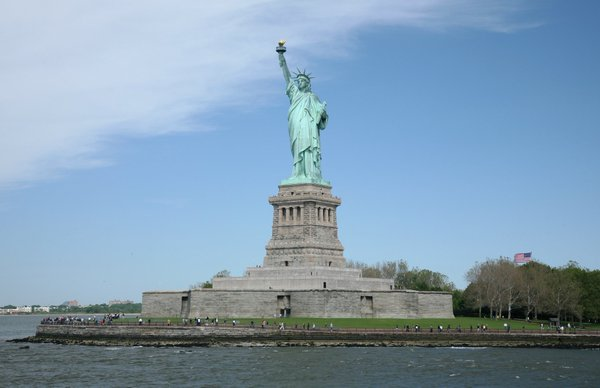
\includegraphics[width=0.927\linewidth]{source.jpg}
		\caption{source.jpg}
	\end{minipage}%
	\begin{minipage}{0.5\linewidth}
		\centering
		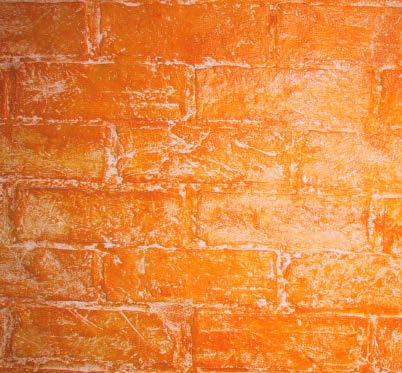
\includegraphics[width=0.8 \linewidth]{target.jpg}
		\caption{target.jpg}
	\end{minipage}
\end{figure}

我们需要从图1中提取主要特征(自由女神像)并以图2作为背景,完成两幅图片的融合。

传统的图像编辑方法 Copy \& Paste 处理这类问题时会表现出明显的不调和,经过 Poisson Image Editing 处理得到的图像有较好的视觉效果。

\subsection{算法描述}

(为方便描述,约定图1为{\heiti 融合图},图2为{\heiti 背景图})

传统的 Copy \& Paste 采用的思路是直接转移{\heiti 融合图}的像素值到{\heiti 背景图},其缺点是直接转移的像素(特别是边界)往往与新背景的特征不同,会造成明显的视觉差异。

Poisson Image Editing 采用的思路是转移{\heiti 融合图}的{\heiti 梯度}到{\heiti 背景图},再在{\heiti 背景图}中利用已有的边界信息重建目标区域的特征,从而完成图像融合。


\begin{wrapfigure}{l}{0pt}
    \centering
    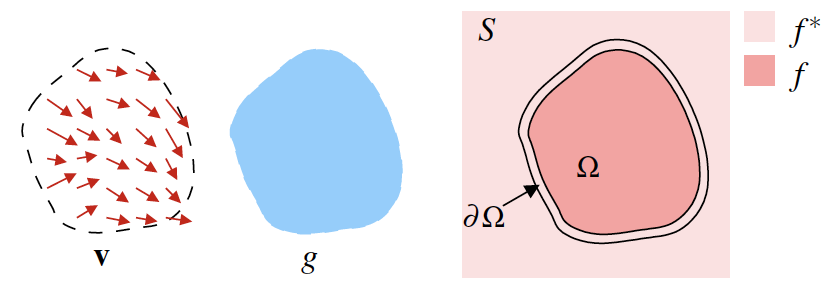
\includegraphics[width=0.62\linewidth]{pic1.png}
    \caption{算法示意图}
\end{wrapfigure}


\noindent
$g$ 表示融合图的提取区域\\
$\mathbf{v}$ 表示目标区域的梯度场\\
$S$ 表示背景图\\
$\Omega$ 表示背景图中待求的融合位置\\
$\partial \Omega$ 表示背景中融合位置的边界\\
$f$ 表示背景图中需要求解的像素\\
$f^{*}$ 表示背景图非融合区域的像素

\hfill


根据转移目标区域的梯度的思想,我们需要完成的最优化问题为:
\begin{equation}
\min\limits_f \iint _\Omega |\nabla f-\nabla \boldsymbol v |^2 \ \ \mathrm{with}\ f|_{\partial \Omega}=f^*|_{\partial \Omega}
\end{equation}

注意到这是一个求泛函极值的问题,由变分法可知该方程的解为:
\begin{equation}
\Delta f= \Delta \boldsymbol v\ \mathrm{over}\ \Omega \ \ \mathrm{with}\ f|_{\partial \Omega}=f^*|_{\partial \Omega}
\end{equation}

其中 $\Delta$ 为拉普拉斯算子 (Laplacian Operator)。


\subsection{程序实现 (Normal Seamless Clone)}

\subsubsection{选定融合区域}

这一部分需要用户提取融合图中的主要特征,需要用 \lstinline{cv2.setMouseCallback} 记录鼠标的选定区域。对于选定的 mask 区域,同时在原图上进行绘制实现可视化交互。
\begin{lstlisting}[language=Python]
if event == cv2.EVENT_MOUSEMOVE:
    cv2.rectangle(image, (x-size, y-size), (x+size, y+size), (0, 255, 0),     -1)
    cv2.rectangle(mask,  (x-size, y-size), (x+size, y+size), (255, 255, 255), -1)
    cv2.imshow(windowname, image)   # 实时移动绘制 mask
\end{lstlisting}

\begin{figure}[ht]
	\begin{minipage}{0.5\linewidth}
		\centering
		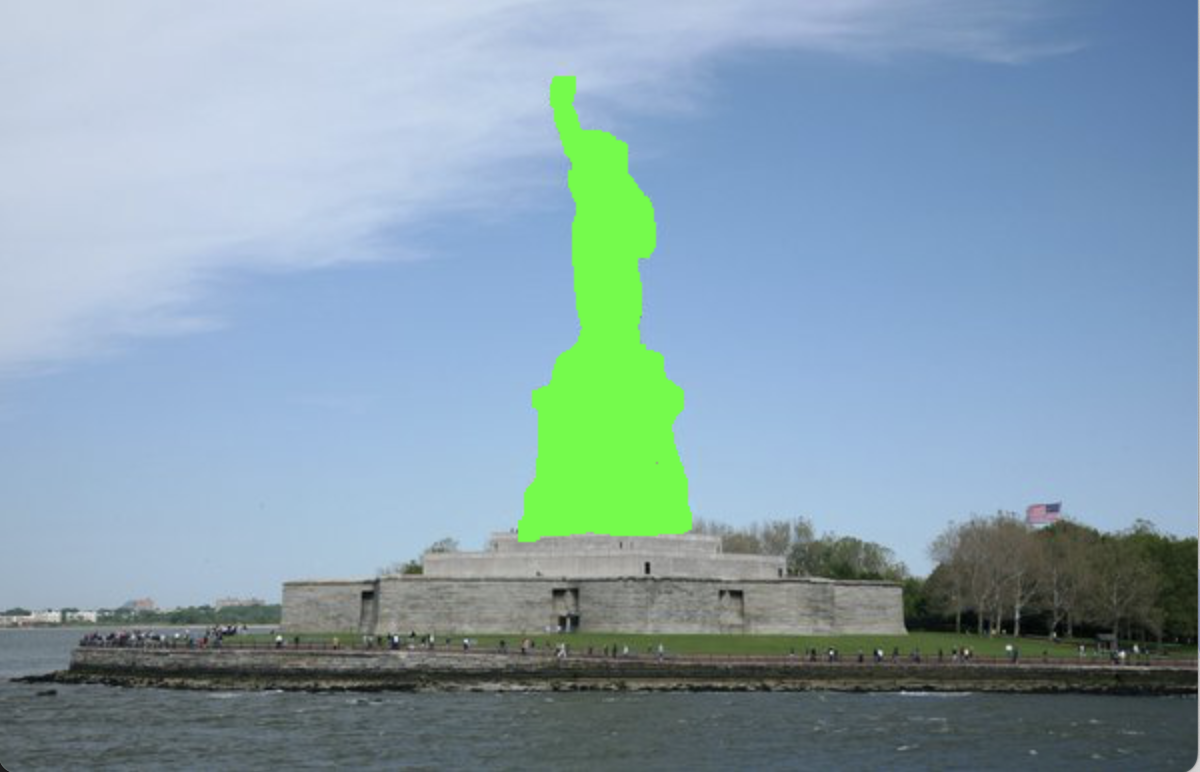
\includegraphics[width=0.8 \linewidth]{source_painted.png}
		\caption{source\_painted.png}
	\end{minipage}%
	\begin{minipage}{0.5\linewidth}
		\centering
		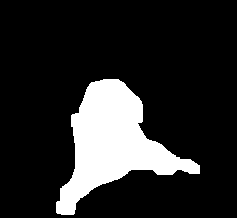
\includegraphics[width=0.8 \linewidth]{source_mask.png}
		\caption{source\_mask.png}
	\end{minipage}
\end{figure}

\subsubsection{选定背景融合区域}

这一部分需要用户将选定区域移动到背景图的某一区域进行融合,同样需要鼠标交互。我们可以在 \lstinline{cv2.setMouseCallback} 记录鼠标移动的参数,求和即为 mask 的偏移量。在这一部分中,可以选择对 mask 每次移动后的结果和背景图进行融合实现可视化。(见图7)

\begin{lstlisting}[language=Python]
if event == cv2.EVENT_MOUSEMOVE:
    M = np.float32([[1, 0, x-x0],
                    [0, 1, y-y0]])
    mask = cv2.warpAffine(mask, M, (mask.shape[1], mask.shape[0]))
    cv2.imshow(windowname, _blend(image, mask))
    # 平移 mask
\end{lstlisting}
\begin{lstlisting}[language=Python]
def _blend(image, mask):
    res = image.copy()
    alpha = 0.7
    res[mask!=0] = res[mask!=0]*alpha + 255*(1-alpha)
    # 融合图像 image : mask = 0.7 : 0.3 
    res = res.astype('uint8')
    return res
\end{lstlisting}


\begin{figure}[ht]
	\begin{minipage}{0.5\linewidth}
		\centering
		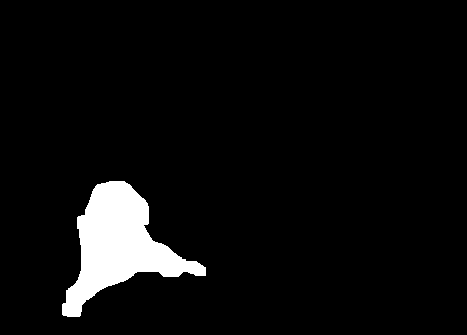
\includegraphics[width=0.8 \linewidth]{raw_target_mask.png}
		\caption{raw\_target\_mask.png}
	\end{minipage}%
	\begin{minipage}{0.5\linewidth}
		\centering
		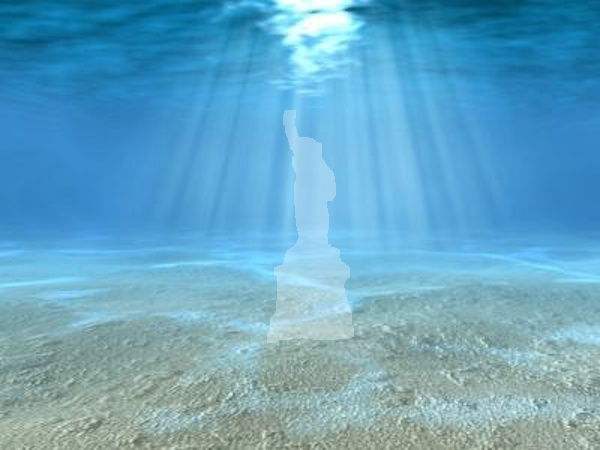
\includegraphics[width=0.8 \linewidth]{mask_blended.png}
		\caption{mask\_blended.png}
	\end{minipage}
\end{figure}



\subsubsection{重建图像}

最后,我们对图像进行重建。对非融合区域的图像,保留背景图中的信息;对融合区域的图像,泊松方程给出了最优解的形式,即 $\Delta f = \Delta g$。

在二维平面中,Laplacian 算子 $\Delta = \frac{\partial^{2}}{\partial x^{2}}+\frac{\partial^{2}}{\partial y^{2}}$。其离散形式为:

\begin{equation}
\begin{aligned}
\Delta f(i, j) &:=\Delta_{i} f(i, j)+\Delta_{j} f(i, j) \\
&=f(i+1, j)+f(i-1, j)+f(i, j+1)+f(i, j-1)-4 f(i, j)
\end{aligned}
\end{equation}

下面以 $m \times n$ 的图像为例,给出一种融合区域的求解办法。

设图像的解 $f$ 为
\begin{equation}
\mathbf{u} = [u_{11}, u_{12}, \dots, u_{1n}, u_{21}, u_{22}, \dots, u_{2n}, \dots, u_{mn} ]^\top
\end{equation}
其中 $u_{ij}$ 表示结果图中第 $i$ 行 $j$ 列的像素。

记 Laplacian 算子的矩阵形式为 $A^{mn \times mn}$, $I^{m\times m}$ 为 $m$ 阶单位矩阵,则有

\begin{equation}
D^{m \times m}=\left[\begin{array}{ccccccc}
-4 & 1 & 0 & 0 & 0 & \cdots & 0 \\
1 & -4 & 1 & 0 & 0 & \cdots & 0 \\
0 & 1 & -4 & 1 & 0 & \cdots & 0 \\
\vdots & \ddots & \ddots & \ddots & \ddots & \ddots & \vdots \\
0 & \cdots & 0 & 1 & -4 & 1 & 0 \\
0 & \cdots & \cdots & 0 & 1 & -4 & 1 \\
0 & \cdots & \cdots & \cdots & 0 & 1 & 4
\end{array}\right]
\end{equation}

\begin{equation}
A^{mn \times mn}=\left[\begin{array}{ccccccc}
D & I & 0 & 0 & 0 & \cdots & 0 \\
I & D & I & 0 & 0 & \cdots & 0 \\
0 & I & D & I & 0 & \cdots & 0 \\
\vdots & \ddots & \ddots & \ddots & \ddots & \ddots & \vdots \\
0 & \cdots & 0 & I & D & I & 0 \\
0 & \cdots & \cdots & 0 & I & D & I \\
0 & \cdots & \cdots & \cdots & 0 & I & D
\end{array}\right]
\end{equation}

最终方程为
\begin{equation}
    A\mathbf{u} = A\mathbf{g}
\end{equation}

可以直接用 scipy.sparse.linalg.spsolve 求解。

对于非融合区域的像素,设为 $\mathbf{u}$,则

\begin{equation}
    \mathbf{u} = f^*
\end{equation}

至此,最终图的所有像素都已给出解。

\subsection{成果展示}

\begin{figure}[ht]
    \centering
    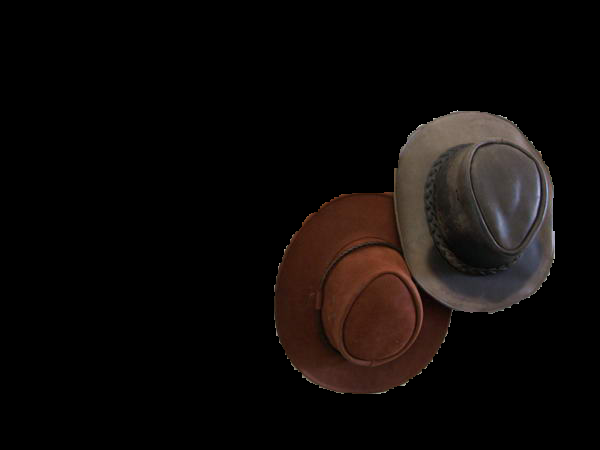
\includegraphics[width=0.6\linewidth]{result.png}
    \caption{result.png}
\end{figure}

\section{算法延伸}

除了常规的图像融合,论文还给出了该算法的一些延伸应用。

\subsection{混合梯度 (Mixed Seamless Clone)}

如果融合图中有洞,或者要将透明的物体添加到有复杂纹理的背景中,得到的图像会有明显的不调和。这是因为透明图的梯度很小,直接选用弱梯度场类似于直接将背景色填充待求的区域。

论文给出了一种混合梯度的解法。即选用融合图和背景图中更强的梯度场,使得融合纹理更鲜明:

\begin{equation}
    \text { for all } \mathbf{x} \in \Omega, \mathbf{v}(\mathbf{x})= \begin{cases}\nabla f^{*}(\mathbf{x}) & \text { if }\left|\nabla f^{*}(\mathbf{x})\right|>|\nabla g(\mathbf{x})| \\ \nabla g(\mathbf{x}) & \text { otherwise }\end{cases}
\end{equation}

\begin{lstlisting}[language=Python]
if mask[y, x] != 0:
    if abs(target_grad_x[y,x,c]) + abs(target_grad_y[y,x,c]) < 
       abs(source_grad_x[y,x,c]) + abs(source_grad_y[y,x,c]):
        target_grad_x[y, x, c] = source_grad_x[y, x, c]
        target_grad_y[y, x, c] = source_grad_y[y, x, c]
        # mixed gradient 按梯度绝对值分配 gradient
\end{lstlisting}

混合梯度往往会比常规的梯度场转移有更优秀的表现。下面是混合梯度和其他方法的效果对比,这里选用的融合图的背景较为单一,背景图的背景纹理复杂。

\begin{figure}[ht]
	\centering
	\begin{minipage}{0.2\linewidth}
		\centering
		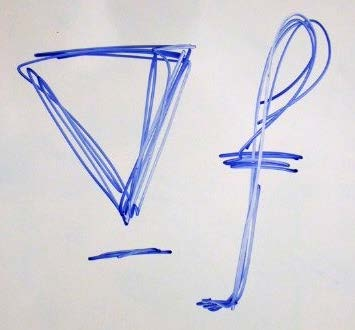
\includegraphics[width=0.97\linewidth]{mixed_source.jpg}
		\caption{mixed\_source}
	\end{minipage}
	\begin{minipage}{0.38\linewidth}
		\centering
		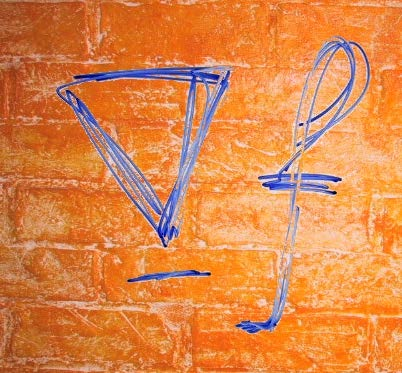
\includegraphics[width=0.97\linewidth]{color-based_result.jpg}
		\caption{color-based cutout and paste}
	\end{minipage}
	\begin{minipage}{0.38\linewidth}
		\centering
		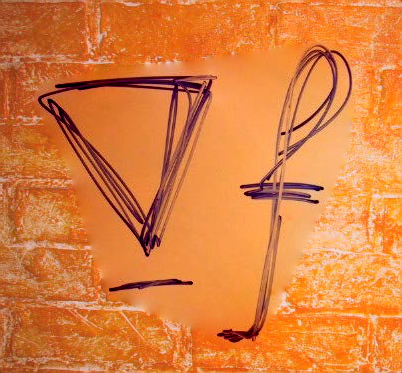
\includegraphics[width=0.97\linewidth]{normal_result.png}
		\caption{normal seamless clone}
	\end{minipage}
	%\qquad
	%让图片换行,
	
	\begin{minipage}{0.2\linewidth}
		\centering
		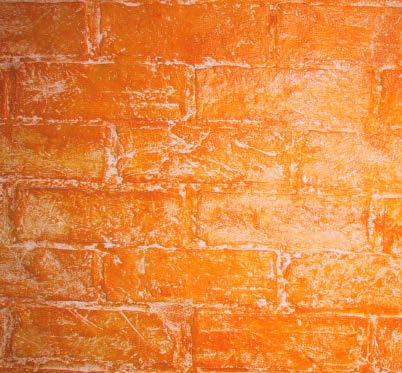
\includegraphics[width=0.97\linewidth]{mixed_target.jpg}
		\caption{mixed\_target}
	\end{minipage}
	\begin{minipage}{0.38\linewidth}
		\centering
		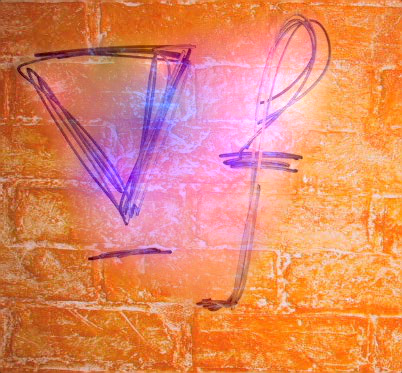
\includegraphics[width=0.97\linewidth]{avg-gradient_result.png}
		\caption{average gradient seamless clone}
	\end{minipage}
	\begin{minipage}{0.38\linewidth}
		\centering
		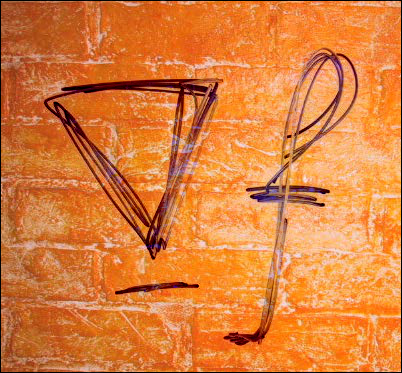
\includegraphics[width=0.97\linewidth]{mixed_result.png}
		\caption{mixed gradient seamless clone}
	\end{minipage}
\end{figure}

\subsection{纹理扁平化 (Texture flattening)}

与上一种延伸算法类似,论文给出了另一种控制梯度场引入的方法,实现了纹理扁平化:

\begin{equation}
    \text { for all } \mathbf{x} \in \Omega, \mathbf{v}(\mathbf{x})= \begin{cases}\nabla g(\mathbf{x}) & \text { if }\left|\nabla g(\mathbf{x})\right| \geq \alpha \\ 0 & \text { otherwise }\end{cases}
\end{equation}

\begin{lstlisting}[language=Python]
if mask[y, x] != 0:
    if abs(source_grad_x[y, x, c]) < alpha:
        source_grad_x[y, x, c] = 0
    if abs(source_grad_y[y, x, c]) < alpha:
        source_grad_y[y, x, c] = 0
    # 消除弱梯度场
\end{lstlisting}

即忽略梯度场中的较小值,下面是这种方法应用的一个例子。

\begin{figure}[ht]
    \centering
	\begin{minipage}{0.35\linewidth}
		\centering
		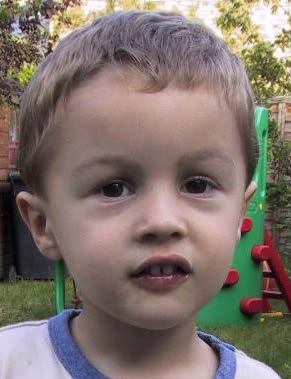
\includegraphics[width=0.7 \linewidth]{flatten_source.jpg}
		\caption{flatten\_source.jpg}
	\end{minipage}%
	\begin{minipage}{0.35\linewidth}
		\centering
		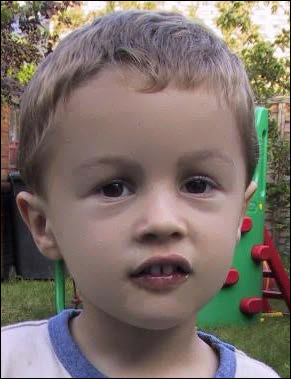
\includegraphics[width=0.7 \linewidth]{flatten_result.png}
		\caption{flatten\_result.png}
	\end{minipage}
\end{figure}

\subsection{局部照明/色彩改变 (Local illumination/color changes)}

局部照明/色彩改变的原理也是调整引入的梯度场。对于局部照明特征的改变,论文给出了梯度场的一种更改规则:

\begin{equation}
\mathbf{v}=\alpha^{\beta}\left|\nabla f^{*}\right|^{-\beta} \nabla f^{*}
\end{equation}

对于局部色彩特征的改变,只需要分别在 R,G,B 三个色彩通道中对梯度进行加权即可。

\section{总结}

传统的图像编辑方法是针对图像的像素进行转移操作,Poisson Image Editing 则是根据图像提供的梯度场进行图像重建。就呈现效果而言,后者得到的结果往往更具真实感,在大部分图像上不会出现明显的视觉差异。

但归根结底,Poisson Image Editing 仍然是一种平滑的图像融合方法,受图像大小和图像本身结构的影响很大,在高分辨率和有复杂纹理的图像的场景下,其方程求解时间和图像准确率表现欠佳。

此外,在程序实现的过程中,也存在着一些细节。例如对于 Normal Seamless Clone 而言,我们可以直接对融合图运用 Laplacian Kernel 进行卷积,直接复制到结果矩阵中,再对结果矩阵中对应背景图中不受影响的区域进行替换,同时修正作用于待求未知数的 Laplacian Matrix 。但这种方法在 Mixed Seamless Clone 中看似可以类推(即对背景图也作用一遍 Laplacian Kernel 的卷积,再根据梯度的绝对值 替换相应的卷积值),但实际上并不适用。这是因为梯度场变化后,变分法在泛函上的作用域不应是独立的两部分,而应该在新得到的梯度场下进行。

在进一步的学习中,笔者发现泊松方程的求解可以用离散傅里叶变换(Discrete Fourier Transform)和离散正弦变换(Discrete Sine Transform)优化,这能显著减少最终图像求解花费的时间。

\end{document}